\section{Relating the Shape of Neural Representations to Decoding}
\label{sec:shape-distance-connection}



In \cref{corollary:new} we saw that the Euclidean distance and Frobenius inner product between $\mbK_X$ and $\mbK_Y$ enjoys a nice interpretation in terms of (average) decoder similarity.
This does not provide a completely satisfactory answer of our original question: What does the \textit{geometry} of a neural representation imply about its function (i.e. decoder performance)?
As discussed in \cref{sec:intro}, comparing neural representations through linear kernel matrices, $\mbK_X$ and $\mbK_Y$, is motivated from geometric principles---namely, their invariance to orthogonal transformations.
Indeed, for any orthogonal matrix $\mbR$, one can verify that:
\begin{equation}
\mbG(\mbX \mbR)^{-1} = \mbR^\top \mbG(\mbX)^{-1} \mbR
\end{equation}
whenever $\mbG(\mbX)$ is parameterized as in \cref{eq:G-alpha-beta}.
Therefore, then the transformation $\mbX \mapsto \mbX \mbR$ leaves the whitened linear kernel matrix unchanged.
That is, if $\mbX^\prime = \mbX \mbR$, we have:
\begin{equation}
\mbK_X = \tfrac{1}{M}\mbX \mbG(\mbX)^{-1} \mbX^\top = \tfrac{1}{M}\mbX \mbR \mbG(\mbX \mbR)^{-1}  \mbR^\top \mbX^\top = \mbK_{X'}.
\end{equation}

The \textbf{Procrustes shape distance}, $\cP(\cdot,\cdot)$, is another popular method which is invariant to orthogonal transformations~\cite{williams2021generalized,Ding2021}.
This approach connects to a broader and decades-old literature on \textit{shape analysis}~\cite{dryden2016statistical,kendall2009shape} whose applications include anatomical comparisons across biological species~\cite{Elewa2004-sb}, and analysis of planar curves such as handwriting data~\cite{Srivastava2016-yq}.
If the two neural responses are mean-centered and have the same dimensionality, then the Procrustes distance is simply the minimal Euclidean distance obtained by rotating and reflecting one set of responses onto the other.
That is, when $\mbX \in \reals^{M \times N_X}$ and $\mbY \in \reals^{M \times N_Y}$ and we have $N = N_X = N_Y$, the Procrustes distance is:

\begin{equation}\label{eq:proc-dist-def}
\cP(\mbX, \mbY) = \min_{\mbR \in \cO(N)} \Vert \mbX - \mbY \mbR \Vert_F
\end{equation}
When $N_X \neq N_Y$, a straightforward generalization of the Procrustes distance is to zero pad column-wise so that the matrix dimensions match.
Geometrically, this can be interpreted as embedding the lower-dimensional point cloud into the higher-dimensional space and optimizing $\mbR$ within this space to align the point clouds.


Some empirical analyses have highlighted cases where using the Procrustes distance turns out to be ``better'' in some sense than linear CKA~\cite{Ding2021,cloos2024differentiable}.
Rigorously defining and benchmarking what it means to be ``better'' in this context remains an open discussion~\cite{klabunde2024resi}, but it is nonetheless of interest to understand what Procrustes distance and associated definitions of \textit{shape} imply about neural decoding.

In \cref{appendix:bounds} we prove the following result, which states that the Procrustes distance between appropriately normalized representations constrains the average decoding distance, or equivalently, that the average decoding distance bounds the Procrustes distance from above and below.


\begin{proposition}\label{proposition:bounds}

Defining normalization constants $\alpha = \Tr \mbK_X$ and $\beta = \Tr \mbK_Y$, we have an upper and lower bound on the Procrustes distance:

\begin{equation}\label{eq:bound_proc}
 (\alpha + \beta) - \sqrt{(\alpha + \beta )^2 - \pr_\Delta \expect \Vert \mbX \mbw^* - \mbY \mbv^* \Vert_2^2} \leq \cP (\tilde{\mbX}, \tilde{\mbY})^2 \le \sqrt{\pr_\Delta \expect \Vert \mbX \mbw^* - \mbY \mbv^* \Vert_2^2}
\end{equation}

where $\pr_\Delta = \pr(\mbK_X - \mbK_Y)$ is the participation ratio of the matrix difference $\mbK_X - \mbK_Y$.
Equivalently, we may rewrite \cref{eq:bound_proc} to find

\begin{equation}\label{eq:bound_euclid}
\frac{1}{\pr_\Delta}\cP (\tilde{\mbX}, \tilde{\mbY})^4 \le \expect \Vert \mbX \mbw^* - \mbY \mbv^* \Vert_2^2 \le \frac{2(\alpha + \beta)\cP (\tilde{\mbX}, \tilde{\mbY})^2 - \cP (\tilde{\mbX}, \tilde{\mbY})^4 }{{\pr_\Delta}},
\end{equation}
where we have defined normalized transformations $\tilde{\mbX}$ and $\tilde{\mbY}$ in terms of the transformation $\mbG(\cdot)$:
\begin{align*}
    \tilde{\mbX} := \tfrac{1}{\sqrt{M}} \mbX \mbG(\mbX)^{-1/2}\quad\text{and}\quad \tilde{\mbY} := \tfrac{1}{\sqrt{M}} \mbY \mbG(\mbY)^{-1/2}.
\end{align*}
Note that $\tilde{\mbX}\tilde{\mbX}^\top = 
\mbK_X$ and $\tilde{\mbY}\tilde{\mbY}^\top = \mbK_Y$.
\end{proposition}


We derive these bounds by leveraging the equivalence between the Procrustes distance between normalized representations $\cP (\tilde{\mbX}, \tilde{\mbY})$ and a distance metric on positive semi-definite kernel matrices, the \emph{Bures distance} \cite{Harvey2024}.  


We recall that the choice of function $\mbG(\cdot)$ in the decoding problem \cref{eq:readout-optimization-class} (which determines optimal readout weights $\mbw^*$ and $\mbv^*$) will set the normalization 
transformation of the representations $\tilde{\mbX}$ and $ \tilde{\mbY}$.
When $\mbG(\cdot)$ is chosen such that $\Tr \mbK_X = \Tr \mbK_Y = 1$,\footnote{For example  $\mbG(\mbX) = N_X\mbC_X$ or the CKA choice from above with $b = \Tr[\mbC_X]$. This is not a requirement for these bounds to hold, but simply a choice of normalization for the sake of plotting.} we can plot these bounds with $\alpha = \beta = 1$ for various values of participation ratio $\pr_\Delta$ (\cref{fig:bounds}).


Both upper and lower bounds are saturated (\cref{appendix:bounds}), and reveal 
an allowed region of both Procrustes and average decoding distance as a function of the participation ratio $\pr_\Delta$.  
Under the $\alpha = \beta = 1$ normalization, the Procrustes distance may range between 0 and $\sqrt{2}$, and the average decoding distance may take values between $0$ and $\frac{2}{\sqrt{\pr_\Delta}}$, which is reflected in \cref{fig:bounds}. 
%
\begin{figure}[t]
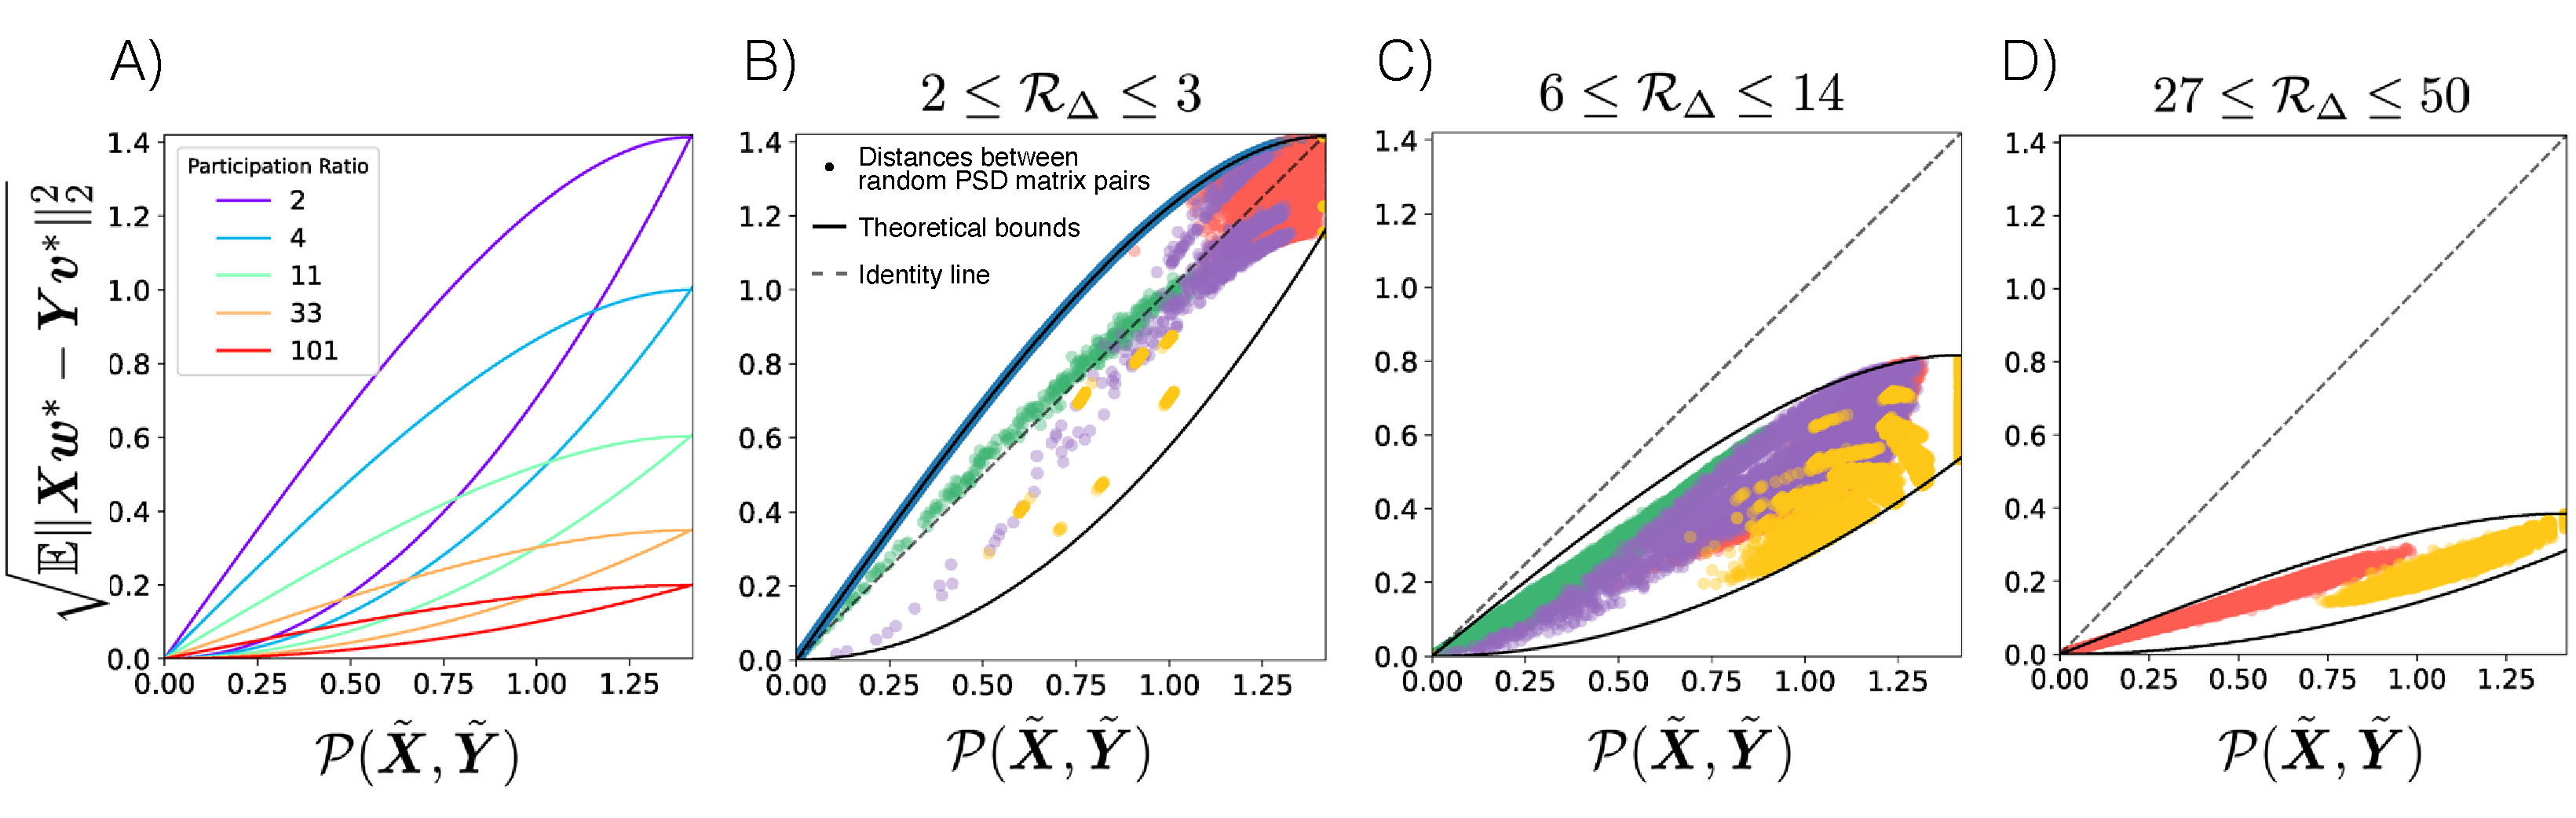
\includegraphics[width=\textwidth]{bound_figure_v6.pdf}
\centering
\caption{Bounds in \cref{eq:bound_proc} plotted (solid lines) for varying participation ratio $\pr_\Delta$ with $\alpha = \beta = 1$.  A)  Allowed regions (between the solid curves of like color) of Procrustes distance and expected Euclidean distance between decoded signals for different values of participation ratio $\pr_\Delta$. B--D) Allowed regions for particular $\pr_\Delta$ intervals (black solid lines) populated with calculated distances between pairs of randomly sampled positive semi-definite (PSD) matrices of size $50 \times 50$, subsampled to those that have $\pr_\Delta$ in the particular interval (colored points). Different colors represent different random ensembles of positive semi-definite matrix pairs, which are described in \cref{appendix:fig2}.}
\label{fig:bounds}
\end{figure}
%

The bounds in \cref{eq:bound_proc} and \cref{eq:bound_euclid} reveal an imperfect connection between the Procrustes distance and the average decoding distance, such as the GULP distance.  
We recall that every choice of readout weight normalization $\mbG(\mbX)$ leads to a measure of representational distance $\expect \Vert \mbX \mbw^* - \mbY \mbv^* \Vert^2_2$, and that there is an associated Procrustes distance on the normalized representations $\tilde{\mbX}$ and $\tilde{\mbY}$, $\cP (\tilde{\mbX}, \tilde{\mbY})$.  
These bounds tell us that the average decoding distance $\expect \Vert \mbX \mbw^* - \mbY \mbv^* \Vert^2_2$ and this Procrustes distance constrain each other in a very particular way.  
Namely, when the Procrustes distance between normalized representations is small, then the average decoding distance must also be small.\footnote{The scale of ``small" and ``large" here are determined by $\alpha$, $\beta$, and $\pr_\Delta$, as the range of the Procrustes distance is between $0$ and $ \sqrt{\alpha + \beta}$, while range of the average decoding distance is between 0 and $\frac{\alpha + \beta}{\sqrt{\pr_\Delta}}$. }  
However, the converse is only necessarily true when the participation ratio of the difference of the kernel matrices $\mbK_X - \mbK_Y$ is also small (e.g.\ \cref{fig:bounds}B).  
Indeed, as the dimensionality of $\mbK_X - \mbK_Y$ increases, we see that the Procrustes distance between normalized representations can be large, but the average decoding distance can be relatively small, with the effect becoming more exaggerated as $\pr_\Delta$ becomes large (\cref{fig:bounds}D).  
In \cref{appendix:bounds} we show that for $\alpha = \beta = 1$, the minimum possible participation ratio $\pr_\Delta$ is 2.  
Therefore, \cref{fig:bounds} also illustrates another interesting phenomenon, namely that the upper left-hand corner of these plots is impossible to populate. 
That is, in the case of large expected difference in decoded signals, one can never simultaneously measure a small Procrustes distance between the normalized representations.
Thus we observe quantitatively, as may be intuitive, that the Procrustes distance offers a more strict notion of geometric dissimilarity than the average decoding distance.  



